\section{Génération des nombres premiers}

	Les cryptosystèmes utilisent une approche commune pour la génération des nombres premiers. Cette approche générale consiste à utiliser un générateur de nombres aléatoires pour générer un entier, dont on testera ensuite la primalité. Ce processus est illustré par la figure ci-dessous :
	
	\begin{figure}[H]
		\begin{center}
		\begin{tikzpicture}
		\begin{scope}
			\node (Gen) at (0,0) [rectangle,draw] {\begin{tabular}{c}Générateur de\\nombres aléatoires\end{tabular}};	
			\node (Test) at (6,0) [rectangle,draw] {\begin{tabular}{c}Test de\\primalité\end{tabular}};	
			\node (Prim) at (10,1) [rectangle] {\begin{tabular}{c}$\bar{p}$ est premier\end{tabular}};	
			\node (Comp) at (10,-1) [rectangle] {\begin{tabular}{c}$\bar{p}$ est composé\end{tabular}};	
			
			\draw[-triangle 45] (Gen) -- node[anchor=south]{Candidat $\bar{p}$} (Test);
			\draw[-triangle 45] (Test) -- node[anchor=south]{} (Prim.180);
			\draw[-triangle 45] (Test) -- node[anchor=south]{} (Comp.180);
		
		\end{scope}
		\end{tikzpicture}
		\end{center}
		\caption{Processus de génération des nombres premiers}\label{fig:M2}
	\end{figure}
	Dans cette démarche, il est important d'utiliser un bon générateur de nombres aléatoires, qui ne doit dans aucun cas être prévisible. Si un attaquant réussit à deviner les nombres premiers qui composent le module RSA, alors le système est immédiatement cassé.

	\subsubsection*{Fréquence des nombres premiers}
	Lors de la génération des nombres premiers à l'aide de ce processus, on voudrait savoir combien de nombres doit-on tester avant de trouver un nombre premier. La réponse à cette question est donnée par le \textit{Théorème des Nombres Premiers}.
	
		\vspace{-1.5em}\begin{adjustwidth}{1.5cm}{1.5cm} 
		\begin{Th}[Théorème des Nombres Premiers]
			Soit $\pi(n)$ le nombre de premiers qui sont inférieurs à $n$, alors
			\[\pi(n) \approx \frac{n}{ln(n)} \quad \quad (n \to +\infty)\]
		\end{Th}
		\end{adjustwidth}\vspace{0.5em}
		
	Un graphique de la fonction $\pi(n)$ pour les 1000 premiers nombres premiers est donné dans la figure ci-dessous :
	\begin{figure}[H]
		\begin{center}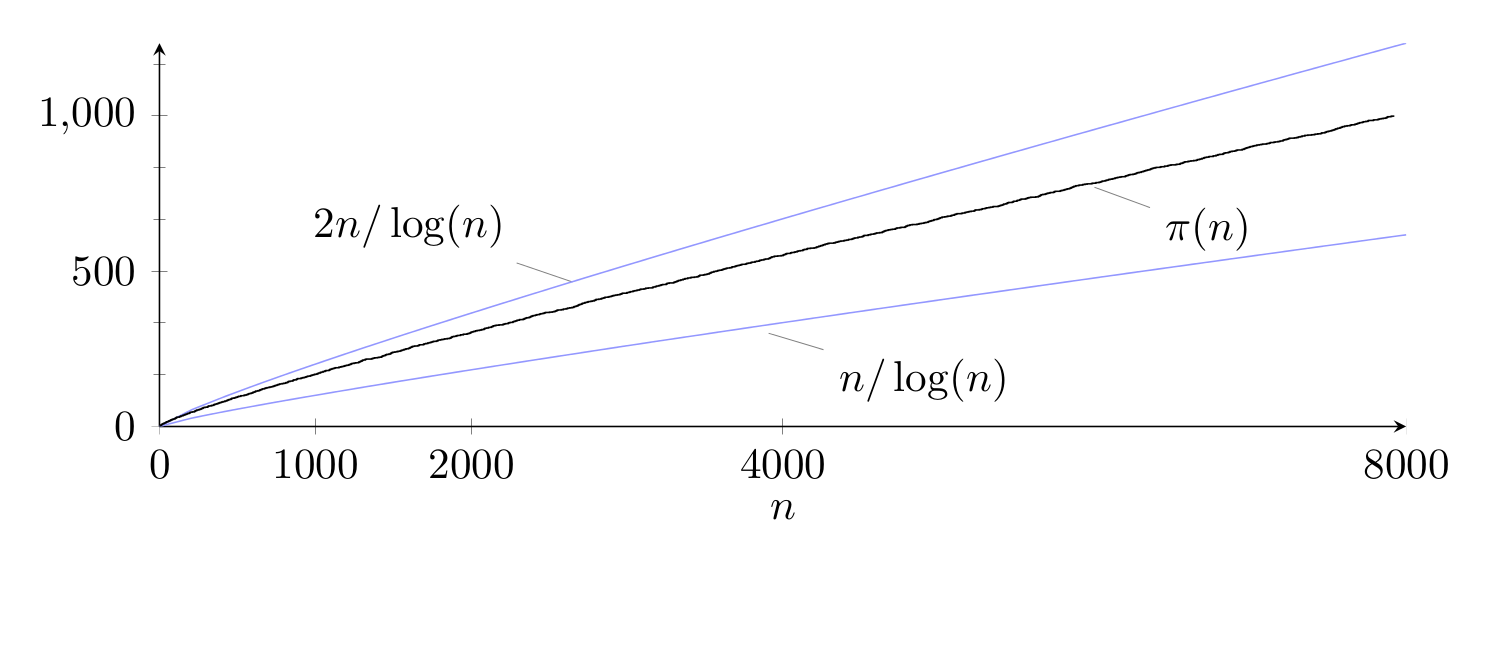
\includegraphics[scale=0.4]{img/freqPremiers.png}\end{center}\vspace{-3em}
		\caption{La fonction $\pi(n)$ pour les 1000 premiers nombres premiers}\label{fig:M3}
	\end{figure}
	
	Le tableau suivant contient l'approximation ainsi que le nombre exact de nombres premiers pour différentes valeurs de $n$. On y remarque que l'approximation est assez bonne.
	\begin{table}[H]\begin{center}
		\begin{tabular}{|lll|}
		\hline
		$n$  & $n/ln(n)$ & $\pi(n)$     \\ \hline
		$10^{3}$ & $145$     & $168$     \\
		$10^{4}$ & $1 086$   & $1 229$   \\
		$10^{5}$ & $8 686$   & $9 592$   \\
		$10^{6}$ & $72 382$  & $78 498$  \\
		$10^{7}$ & $620 420$ & $664 579$ \\ \hline
		\end{tabular}
	\end{center}\end{table}
	
	\paragraph{Probabilité de générer un nombre premier $p$ de $k$ bits :} on sait que $2^{k-1} \leqslant p \leqslant 2^{k}-1$. Le nombre de nombres premiers dans cet intervalle (c-à-d de $k$ bits) peut être approximé par :
	\[ \pi(2^{k}) - \pi(2^{k-1}) \approx \frac{2^{k}}{ln(2^{k})} - \frac{2^{k-1}}{ln(2^{k-1})} \approx \frac{2^{k-1}}{ln(2^{k-1})}	\]
	puisque $ln(2^{k}) = ln(2.2^{k-1}) = ln(2) + ln(2^{k-1})$, donc $ln(2^{k}) \approx ln(2^{k-1})$ pour $k$ grand.
	\vspace{1em}
	\\
	\noindent Donc, il y'a $2^{k-1}$ entiers $\in [2^{k-1},2^{k}-1]$ (de $k$ bits) dont approximativement $\frac{2^{k-1}}{ln(2^{k-1})}$ parmi eux qui sont premiers. Par conséquent, un nombre $p$ de $k$ bits sera premier avec une probabilité de :
	\[\frac{1}{ln(2^{k-1})}\]
	
	\paragraph{Cas de RSA-1024 :} pour générer une des deux clé de RSA-1024 dont la taille en bits est 512, on a probabilité de $1/ln(2^{511}) \approx 1/355$ pour générer un nombre premier de 512 bits. Cette chance double si on se restreint sur les entiers impairs, c'est à dire qu'on doit générer à peu près 177 nombres avant de tomber sur un nombre premier.